\chapter{Automated neuroimaging data management with the Sea filesystem}

Val\'erie Hayot-Sasson and Tristan Glatard \\
\begingroup \footnotesize
Department of Computer Science and Software Engineering, Concordia University, Montreal, Canada \\
\endgroup 
\vspace{5pt} \\
In preparation: \\

\section{Abstract}
	Neuroimaging open-data initiatives have led to the availability of large scientific datasets. These voluminous
	datasets provide researchers with new insights into the human brain across diverse populations. Difficulties with
	managing such large data has partially hindered the advancement of scientific studies analyzing these datasets. Many
	software tools and strategies have emerged to facilitate the processing. Many open datasets have been stored on cloud storage
	services, such as AWS, enabling rapid transfer of the data at a cost\todo{What cost?}. Software tools such as Datalad has facilitated both the
	sharing and versioning of data. Despite these advancements in-analysis data-management remains limited in neuroimaging workflows.
    
	Neuroimaging workflows, particularly preprocessing ones, may lead to a magnification in output sizes due to <add reason>. They also produce
	significant amounts of intermediary data due to being composed of a multitude of steps. 
    \todo{this sounds a lot like an intro that teasing about general context, not an abstract that summarize the chapter}

    \section{Introduction}\label{sec:sea_neuro:introduction}
    
    Neuroimaging datasets continue to grow in size resulting in new challenges related
    to data management. The current largest neuroimaging datasets, such as the Human Connectome Project (HCP)~\cite{HCP}
    and the UK Biobank~\cite{ukbiobank} reach up to Petabytes of data. Big Data in neuroimaging can be present in two formats: 1)
    very large files, such as those found in the BigBrain~\cite{bigbrain}, and 2)\todo{what is that 2?} large datasets made up of very small files,
    such as those typically found in fMRI datasets. 
    
    When processing, large datasets can result in longer processing times even when compute resources are ample.
    This is a direct result of the underlying storage used by the applications to read and write data. Since large
    datasets require a significant amount of available storage space, more often than not, slower but larger storage is
    selected, resulting in longer data transfer times during processing. With the Sea filesystem, we aim to
    leverage all available storage in order to reduce overall data transfer time during pipeline execution.
    
    Many researchers rely on one of two systems to meet their storage and computing needs: 1) High Performance 
    Computing (HPC) clusters and 2) the cloud. Whereas the cloud simplifies data sharing and gives researchers
    access to a wide variety of infrastructures, HPC clusters are a cost-effective solution to accessing a wide
    array of resources for researchers. In this paper, we will focus on HPC processing.
    
    HPC systems rely on scalable network-based parallel filesystems (e.g. Lustre) for storage. While such file
    systems offer excellent performance, they are shared between all the users on the cluster. Meaning that users
    with data-intensive can effectively deteriorate the performance of the shared file system for all users on
    the cluster. Solutions for improving shared file system performance include throttling the data intensive workloads
    or recommending the use of Burst Buffers~\cite{bb} (e.g. reserving a compute node for storage or leveraging
    local compute storage during processing). The latter, however, requiring that the user manages their data to
    and from the Burst Buffer.
    
    Leveraging local storage to improve data intensive workload performance has long since existed in Big Data
    frameworks such as Apache Spark~\cite{spark} and Dask~\cite{dask}. While these frameworks have been used to
    process neuroimaging data~\cite{manypapers}, they remain seldom used as their require rewriting existing
    standard neuroimaging tools (e.g FSL, AFNI, SPM) for the framework. Although it is possible to use the
    tools within the Big Data frameworks, optimizations like in-memory computing would not be leveraged due to 
    the fact that neuroimaging tools are meant to be used as command-line tools and do not provide interfaces that 
    enable the data to be transferred in-memory.
    
    Frameworks used in neuroimaging, such as NiPype~\cite{nipype} and Joblib~\cite{joblib} instead focus on reducing compute times of workloads.
    This is because even with large datasets, neuroimaging data processing remains split between compute and data
    intensive components. Although these frameworks do not prohibit the use of intelligent data management, it is not directly integrated
    into the workflow. In order to give neuroimaging applications data management capabilities, the applications must interact with a
    file system that can do so.
    
    In order for a file system to be usable by the average researcher on an HPC system, they must be loadable without administrative
    privileges. Furthermore, as the applications are typically made to interact with POSIX-based file systems, the new file system must
    also be compliant to the format. One method to ensure that these conditions are met is by using the \texttt{LD\_PRELOAD} trick. This trick is
    used to intercept select library calls and redefine their behaviour. It has been used in many projects and to create lightweight versions
    of filesystems~\cite{xtreemfs}. 
    
    In this paper, we present Sea, a file system designed to automate data management of neuroimaging pipelines running on HPC systems.
    The goal of Sea is to complement existing neuroimaging applications such that both efficient compute and data management can be achieved
    executed on HPC without significant user intervention. As a secondary goal, Sea aims to ensure the fair sharing of cluster usage
    by alleviating the impacts of heavy writers on the shared file systems as a whole. 
    
    
    
    % \section{Related Work}
    
    % Put in intro.
    % summary of computing landscape for neuroimaging.
    % HCP, CBRAIN, nipype, joblib. sea can be used in all these contexts.
    
    
    \section{Materials and Methods}
    
    \subsection{The Sea filesystem}
    
    The Sea file system is an on-demand file system that leverages the \texttt{LD\_PRELOAD} trick to intercept POSIX file system (more specifically, glibc)
    calls on Linux systems. This enables Sea to redirect write calls aimed for a slower storage device to a faster device whenever
    possible. Similarly, when intercepting read calls, Sea can choose to read from a faster device if a copy is available on that device.
    Sea decides which storage location it can write to based on the detailed provided in an initialization file called \texttt{sea.ini}. 
    This file informs Sea of which locations it can use to read and write to, and well as their order of priority. An example of the initialization
    file can be seen in ~\ref{seaini}\todo{Figure table,link?}.
    
    As neuroimaging pipeline results are typically required post-processing and HPC compute-local resources are only accessible during the
    reserved duration, Sea provides functionality to flush and evict data to persistent shared storage. This is accomplished via a separate
    thread (known as the ``flusher'') that moves data from the caches to long-term storage. A separate thread is used, in this case, to avoid
    interrupting on going processing with data management operations.
    Users must inform Sea of files that need to be
    persisted to storage within a file called \texttt{.sea\_flushlist}, and temporary files which can be removed from cache within a file
    called the \texttt{.sea\_evictlist}\todo{I would have used .config/sea/evictlist, as user it is better to handle.}. Both these files can be populated using regular expressions to denote the paths to flush and evict.
    If a file occurs in both the \texttt{.sea\_flushlist} and \texttt{.sea\_evictlist}, Sea will interpret this as a \texttt{move} operation
    and simply move the file from local to persistent storage rather than copying it. Files that will be reused by the application should only
    be flushed rather than flushed and evicted, as files can benefit from speedups related to reading from fast rather than slow storage.
    Sea currently also provides a rudimentary prefetch thread that can move files located within the Sea filesystem to the fastest available cache.
    To use Sea's prefetch capabilities, a file called \texttt{.sea\_prefetchlist} needs to be populated using regular expressions like the
    flushing and eviction files.
    
    To interact with the Sea file system, a mountpoint is used. The mountpoint is an empty directory that behaves as a view to
    all the files and directories stored within Sea. In order to keep track of the locations of the files within the mountpoint, Sea
    mirrors the file structure of each storage location across all storage locations. That means, it is generally advisable to provide
    empty storage locations for Sea to write to as the mirroring of large directories can take some time. When prefetching, it is
    best to provide Sea with a path that only points to that data the requires prefetching as mirroring the paths of full datasets may 
    extend processing time.\todo{maybe move that earlier. Overall, this paragraph is not clear. Does sea copies everything from all its mounted point?}
    
    Sea can easily be launched\todo{launched or tested?} directly using the available containers on the GitHub registry, or can be compiled via source using Make.
    It requires a version of glibc greater than X\todo{what is X? 10?}. Once compiled, Sea can be executed using the `sea-app.sh' binary\todo{that doesnt look like an LDPRELOAD. Also, you can give a link to Sea's readme.}.
    
    \subsection{Performance analysis of Sea for neuroimaging}
    
    To determine the performance gain Sea brings to neuroimaging analyses, we must evaluate the value of Sea on a variety of neuroimaging
    applications. For our analysis, we selected different fMRI preprocessing applications as fMRI processing has some of the most
    well-established tools for neuroimaging and some of the largest datasets. Of course, different modalities an tools may result in
    vastly different data access patterns and compute times, we use fMRI prepreprocessing as our baseline for the benefits that can be
    obtained with Sea. 
    
    
    
    \subsubsection{Datasets}
    fMRI datasets may vary greatly in total number
    of images and number of volumes within each image. To adequately capture the 
    diversity of datasets and the applicability of Sea, we have selected three datasets of varying
    time and space resolutions (Table~\ref{table:data}): 1) OpenNeuro's ds001545 dataset~\cite{ds001545},
    2) the PREVENT-AD dataset~\cite{preventad}, and 3) the HCP dataset~\cite{HCP}.
    The ds001545 dataset is a total of 45.94~$GB$ (1778 files) and consists of data collected
    from 30 participants in a single session watching 3 different clips (i.e. three runs/participants) of the The Grand Budapest Hotel.
    
    
    The PREVENT-AD dataset is publicly available dataset comprising of data from 330 participants with a familial history
    of Alzheimer's Disease.
    At the time of the experiments, the dataset contained 255.0~$GB$ (53061 files) originating from the 308 subjects available on DataLad~\cite{}.
    
    The HCP project, whose aim is to characterize brain connectivity using data collected from 1200 subjects, is the largest of the three datasets.
    At the time of our experimments, the dataset obtained consisted 85.4~$TB$ (x files\todo{what is x? 10?}) of data collected from 1113 subjects.
    
    By experimenting with datasets of different spatial and temporal resolutions, the amount of compute may be affected.
    Naturally, with more data there may inevitably be more computations performed, but also, the code itself may
    chose to perform entirely different computations as a result of differences in resolution. Moreover, parallelism and program I/O behaviour
    may be impacted depending on the particular characteristics of the data. Capturing this potential
    variety in processing will provide us with a better understanding of when and where Sea can be useful.
    
    \begin{table*}[t]
      \small\centering
    \resizebox{\textwidth}{!}{\begin{tabular}{|c c c c c|}
      \hline
      Dataset & Total Size (MB) & Total Number of images & Number of images processed & Total size of processed (MB) \\
      \hline
      \multirow{3}{*}{PREVENT-AD} & \multirow{3}{*}{289532} & \multirow{3}{*}{53061} & 1 & 51.26\\
      & & & 8 & \\
      & & & 16 & \\
      \hline
      \multirow{3}{*}{ds001545} & \multirow{3}{*}{27377} & \multirow{3}{*}{1778} & 1 & 280.27\\
      & & & 8 & \\
      & & & 16 & \\
      \hline
      \multirow{3}{*}{HCP} & \multirow{3}{*}{83140079} & \multirow{3}{*}{X} & 1 &  1299.93\\
      & & & 8 & \\
      & & & 16 & \\
    
    
      \hline
    
      \hline
    \end{tabular}}\caption{Dataset characteristics}\label{table:data}
    \end{table*}
    
    %just for example run
    %dataset size, resolution, resolution of voxels
    %matrix size pixdim1X2
    %number of slices pixdim
    %number of volumes pixdim4
    %inplane resolution pixsize1x2
    %slice thickness pizsize3 in mm
    %repetition time pixsize4 in s
    
    %HCP resting state + x stats
    
    %# files written and output size, duration and memory consumption.
    \subsubsection{fMRI Preprocessing Pipelines}
    
    Similarly to datasets, preprocessing pipelines can also vary in duration as a result of methodological differences.
    Thus, we preprocessed each dataset using four standard preprocessing pipelines: FSL~\cite{fsl}, AFNI~\cite{AFNI},
    SPM~\cite{spm}, fMRIPrep~\cite{fmriprep}. Table~\ref{table:pipelines} provides an reference of the differences in computation and data-intensivity
    of the different pipelines on a single subject of all three of the datasets \todo{this sentence is complicated, but i forgot why}.
    
    Each tool was set to only run the preprocessing pipeline. Scripts used to execute each pipeline can be found at~\ref{github.com/valhayot/sea-slurm-scripts}.
    
    For the FSL preprocessing pipeline, the default settings were maintained with the exception of slice-timing correction (interleaved),
    intensity normalization and non-linear registration to standard space.
    
    %% Add SPM here
    To preprocess the datasets with SPM12, we reused the template described in \cite{haitas2021}, with fieldmap correction removed.
    As the template was designed for a specific dataset, we updated the paths to the fMRI and anatomical images,
    as well as the dimensions, such as the number of volumes and slices and the TR and TA, for each dataset. Furthermore,
    we set the slice order to interleaved in all cases. 
    
    For AFNI preprocessing, the pipeline was configured to perform slice timing, alignment to Talaraich space, registration, smoothing
    and brain masking. While AFNI does have some parallelized components that can be controlled via environment variables, we chose to let 
    the pipeline use as much parallelism as required for its execution.
    
    We set fMRIPrep to run with \texttt{--fs-no-reconall} flag set and set the \texttt{--bids\-database-dir} to a tmpfs location. 
    Furthermore, the seeds were fixed to ensure reproducible results. Unlike the other tools where only a single fMRI image was preprocessed
    per process, it was not possible to do so with fMRIPrep. Thus, fMRIPrep preprocessed entire subject directories at a time

    %%{provide subject #/session#} of the ds001545 dataset.
    
    \begin{table*}[t]
      \small\centering
      \resizebox{\textwidth}{!}{\begin{tabular}{|c c c c c c|}
      \hline
      Tool & Dataset &  Output Size (MB) & Total libc calls & Libc Lustre calls & Compute time (s) \\
      \hline
      \multirow{3}{1em}{AFNI} & PREVENT-AD & 539.6 & 272390 & 4348 & 103.25 \\
      & ds001545 & 3063.4 & 281707 & 4570  & 280.30 \\
      & HCP & 18720.4 & 305310 & 5367 & 816.16 \\
      \hline
      \multirow{3}{1em}{FSL Feat} & PREVENT-AD & 253.7 & &  & 1338.29 \\
      & ds001545 & 550.6 & &  & 2145.96 \\
      & HCP & 1607.9 & & & 6596.46 \\
      \hline
      \multirow{3}{1em}{SPM} & PREVENT-AD & 331.0 & 34868 & 10048 &  483.67 \\
      & ds001545 & 744.4 & 47251 & 19568 & 446.53 \\
      & HCP & 2082.5 & 54753 & 25226 & 715.43 \\
    
      \hline
    \end{tabular}}\caption{Pipeline execution characteristics}\label{table:pipelines}
    \end{table*}
    \subsection{Controls}
    Our objective is to measure the speedup brought by Sea on real neuroimaging pipelines.
    Although Sea is agnostic to the internals of the pipelines and their output results, incorrect parameter
    selection and resulting outputs may result in I/O patterns that would not necessarily be observed had the
    pipeline been executed properly.
    
    Visual QC on the pipeline to ensure it was correctly registered and skull-striped to the template brain (MNI template). 
    
    To validate that the outputs produced were sufficiently correct, we overlayed the output on the input image.
    This allowed up to see if steps such as skull-stripping and registration were correctly performed on the data.
    We repeated this step for all datasets and all pipelines processing a single image. In addition, we compared output
    number of files and output size to ensure that the pipeline was not producing different outputs depending on the file
    system used.
    
    % compare md5sums of uncompressed files.
    
    \subsection{Infrastructure}
    
    Our experiments were exected on two different clusters: 1) a local cluster and 2) Compute Canada's Beluga cluster.
    The local cluster comprised of 8 compute nodes with 256GB memory and 125GB tmpfs, running Centos 8. Storage on the local
    cluster was comprised of 4 Lustre ZFS storage nodes with 44 HDD OSTs and 1 MDS with a single MDT. The
    storage nodes were connected to the compute nodes via a 20Gbps ethernet connection.
    The cluster's hardware is similar to that of Beluga.
    
    The Beluga cluster consists of a total of 977 compute nodes, of which we used their general compute nodes with 186~$GiB$ of available
    memory, 480~$GiB$ of scratch SSD space, 2 Intel Gold 6148 Skylake @ 2.4 GHz CPUs and Centos 7 installed. Each compute node is connected
    to the Lustre scratch filesystem via an Mellanox Infiniband EDR (100 Gb/s) network interconnect. The scratch filesystem consists of a total 2.6~$PiB$
    of space, with 38 OSTs of 69.8~$TiB$ each and two MDTs of 3.3~$TiB$.
    \todo{normalize si formatting everywhere}

    In our controlled local cluster, we ran the experiments with and without lustre deteriation, which we refer to as busy writers. Without
    busy writers, the neuroimaging pipelines have exclusive access to the cluster. With busy writers, the neuroimaging pipelines are executed alongside
    a Spark application that reads and writes approximately 1000 617MB blocks using 64 threads multiple times (until the neuroimaging applications completes),
    with a 5 seconds sleep between reads and writes. In our experiments, we either had 6 nodes each executing the Spark application or no busy writers.

    To ensure that system performance was equivalent between Sea and baseline, we executed Sea and baseline pipelines together, for all experiments.
    
    %Busy writers
    \section{Results}


\begin{figure*}

\begin{subfigure}{\textwidth}
    \centering
    \captionsetup{width=.85\linewidth}
    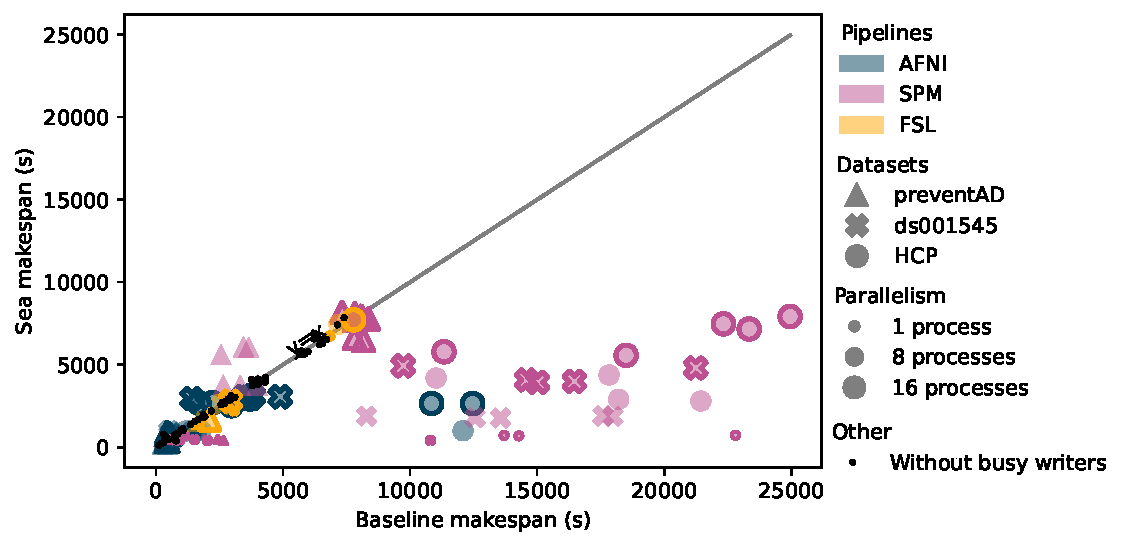
\includegraphics[width=\columnwidth]{figures/sea-neuro/slashbin_results.pdf}%
    \caption{Complete results}\label{fig:seaneuro:slashbinfull}
\end{subfigure}
\begin{subfigure}{\textwidth}
    \centering
    \captionsetup{width=.85\linewidth}
    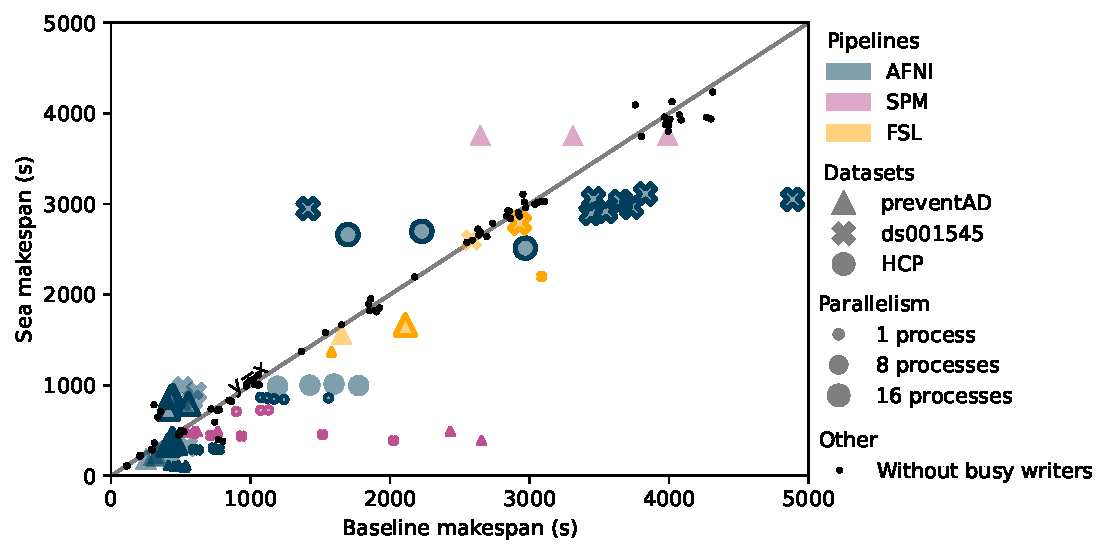
\includegraphics[width=\linewidth]{figures/sea-neuro/slashbin_results_zoomed.pdf}
    \caption{Zoomed between 0 and 5000 seconds}\label{fig:seaneuro:slashbinzoom}
\end{subfigure}
\caption{Makespan comparison between Sea and Baseline on controlled local cluster}
\label{fig:seaneuro:slashbin}
\end{figure*}

In Figure~\ref{fig:seaneuro:slashbin}, we see that although baseline's makespan increases with the presence of busy writers,
Sea's makespan remains relatively stable respective to the dataset and pipeline used. AFNI is has a significantly shorter makespan
than SPM, regardless of the presence of busy writers and dataset type. However, makespan in AFNI is naturally influenced by the presence of both.

For both pipelines, PREVENT-AD has the shortest makespan, with parallelism being a determining factor for speedup. For instance, if we look
at \ref{fig:seaneuro:slashbinzoom}, when using a single process, Sea appears to be consistently faster than baseline for both pipelines.
When we increase the level of parallelism to 8 pipeline processes, whereas Sea is still consistently faster than baseline for AFNI, this
is no longer true for SPM. Interestingly enough, baseline appears to outperform itself with 6 busy writers at 8 parallel processes, whereas
this is not the case at 16 parallel processes. At 16 parallel processes, Sea and Baseline perform almost identically for both SPM and AFNI.

In the case of ds001545, the next smallest dataset, Sea is faster than baseline with SPM for all parallel conditions, with a maximum speedup of 25.8~X~\todo{verify that there was no failure here as average is 3x} at 1 image.
Average speedup was found to be 4~X and 2~x for 8 and 16 threads, respectively. A possible reason for diminishing speedup with increased number of 
threads is that each process may be competing for compute resources as we did not restrict the number of parallel threads.
AFNI, on the other hand, experiences a speedup with Sea at 1 (1.7~X) parallel processes, but a slight slowdown (0.96~X) at 8 parallel processes.
At 16 parallel processes, Sea and Baseline perform similarly. A possible explanation for the slowdown at 8 processes may be related to a memory bottleneck. That is, with the increase in data occupying memory space and additional memory required by the processes, there may be additional data transfers occuring at the CPU-level as a result of initial data placement.

Similarly, HCP, the largest dataset, experienced greater speedups with SPM than with AFNI. Average speedups with
SPM were found to be 6.8~X, 2.7~X and 1.8~X, for 1, 8 and 16 parallel processes, respectively. Speedups with AFNI
were found to be 1.2~X, 2.3~X and 1.6~x at 1, 8 and 16 parallel processes. Unlike with ds001545, AFNI does not experience a slowdown with Sea at 8 parallel processes, possibly due to page cache being overloaded with baseline as a result of the data size and frequency of the writes.



\begin{figure*}

\begin{subfigure}{\textwidth}
    \centering
    \captionsetup{width=.85\linewidth}
    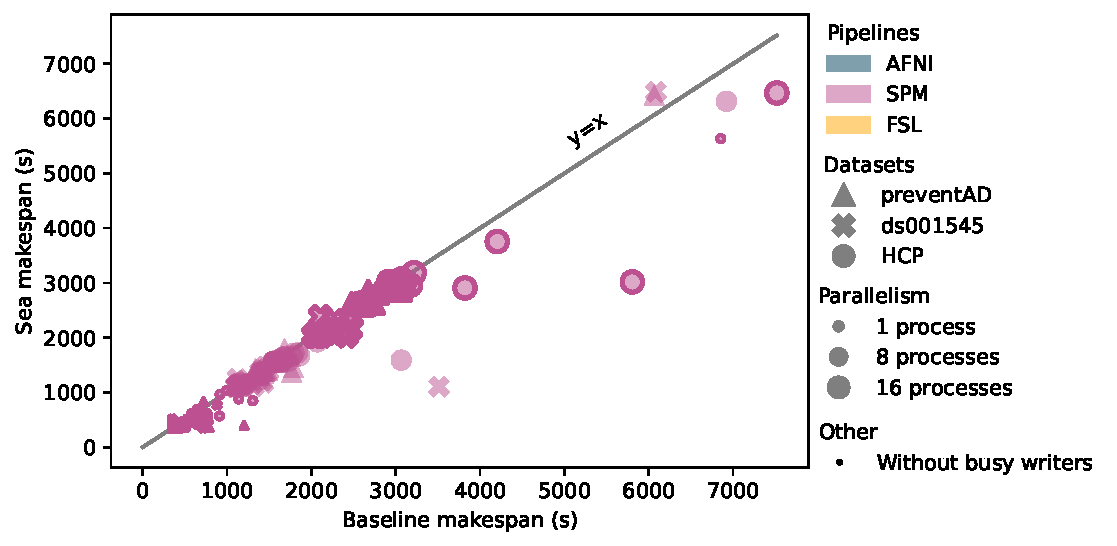
\includegraphics[width=\columnwidth]{figures/sea-neuro/beluga_sea_all.pdf}%
    \caption{Complete results}\label{fig:seaneuro:belugafull}
\end{subfigure}
\begin{subfigure}{\textwidth}
    \centering
    \captionsetup{width=.85\linewidth}
    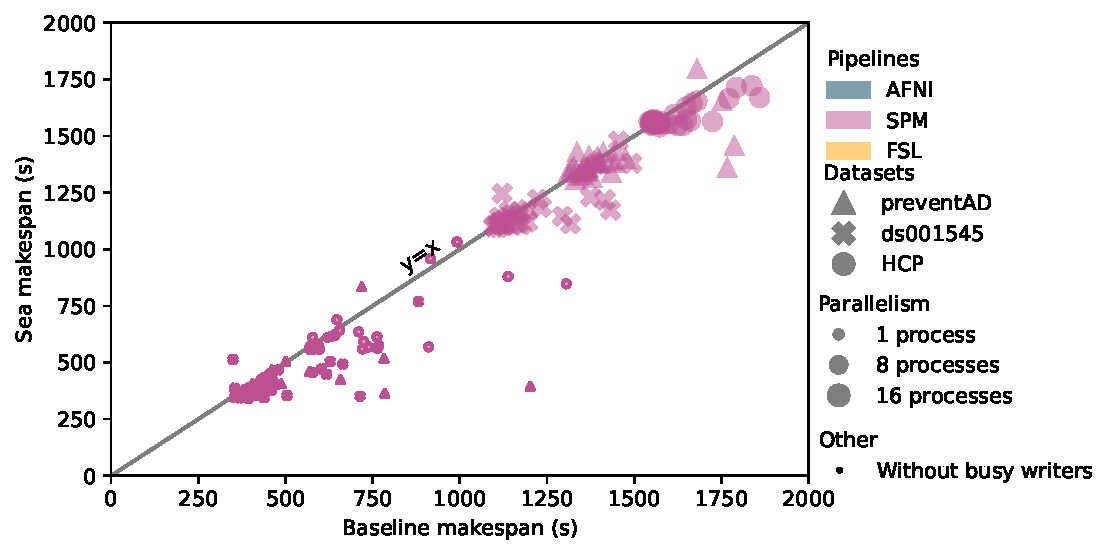
\includegraphics[width=\linewidth]{figures/sea-neuro/beluga_sea_zoom.pdf}
    \caption{Zoomed between 0 and 2000 seconds}\label{fig:seaneuro:belugazoom}
\end{subfigure}
\caption{Makespan comparison between Sea and Baseline on Beluga}
\label{fig:seaneuro:beluga}
\end{figure*}

The Beluga results (Figure~\ref{fig:seaneuro:beluga}), 
shows that Sea and Baseline generally performed 
similarly, but that occassionally, we can obtain large 
speedups with Sea, presumably when Lustre is 
overburdened. The largest speedup obtained by the use of
Sea is 3.2~X which occurred when running SPM on ds001545 with 8 parallel processes. The greatest
slowdown experienced from using Sea was found to be 0.7~X, which occurred when running SPM on ds001545 with a single process. 

    
    
    \section{Discussion}
    \subsection{Significance of speedups with Sea}

    Our results show that the speedups obtained from
    using Sea can be quite substantial (up to 25.8~X)
    depending on the deterioration of the Lustre
    filesystem. On a production cluster where Lustre I/O could not be controlled, we obtained a maximum speedup of 3.2~X.

    While in the average case, Sea and Baseline performed similarly, it is impossible for the
    average cluster user to know if Lustre's performance
    will be deteriorated during the lifetime of their
    application execution. The fact that Sea and Baseline perform similarly in the average case is indicator that runtime is generally not
    deteriorated by Sea and is safe to use in the event where Lustre performance is sufficiently deteriorated.

    Although Sea did result in performance deterioration at times, the magnitude of deterioration is significantly less than that of possible speedups obtained. Our controlled experiments demonstrate that using Sea with a deteriorated Lustre filesystem can result in average speedups of up to 2.6~X. Such results indicate that the risk of a slowdown with Sea are less important that the potential speedups that can arise.

    \subsection{Limitations of using Sea}
    
    Sea really shines when it is executed on a data intensive pipeline.
    This means, the data is written at a rate which exceeds the rate at
    which the compute node's page cache can flush results to Lustre. In
    our experiments, the pipeline which consisted of both the shortest
    duration and largest output size was AFNI processing HCP with 16 subjects.
    While it wrote approximately 100~$GB$ of data, the controlled cluster would
    have had approximately 44~$GB$ of dirty cache available per OST and a maximum
    amount of 100~$GB$ of page cache. Since all writes would not have occurred at the same time
    and computation time was extended as a result of CPU contention, even our controlled experiments
    do not showcase the benefits of Sea in a highly data intensive scenario. However, HCP is one of the largest fMRI datasets, thus the only way to augment data intensitivity of the applications is through increased parallelism which is limited by the number of available cores. As a result, we can
    only demonstrate the speedups brought by Sea when Lustre performance has been deteriorated.


    Sea may not be ideal in instances where there is a memory bottleneck, for instance, as speculated
    with AFNI and ds0015454 using 8 parallel processes on our local cluster. In these experiments, Sea wrote the majority of the results to tmpfs space.
    Since the applications also require a substantial amount of memory space,
    this may have resulted in increased CPU communication. In these cases, it
    is likely preferred to reduce the amount of tmpfs space used by Sea and
    favour writing to disk instead. However, in instances where Lustre
    performance is quite good, we would expect a performance degradation from
    using disk.


    %\subsection{Sea uses more memory}
    %\subsection{Other use cases}
    %writes a lot but it's actually more complicated. When dataset increases
    \subsection{Predicting speedups}

    Our results expose the complexities of performance predictions on a
    production cluster. We present results on a local cluster with which we have
    control over the global cluster usage and are able to demonstrate that
    significant speedups can be obtained when all the disks associated to Lustre
    are busy writing other data concurrently. However, even these experiments
    are limited in demonstrating potential speedups with Sea as there are many
    controlled variables, some of which may vary from cluster to cluster. For
    example, Beluga has a total of 977 nodes and only 38 disks associated with
    their Lustre scratch file system. We can imagine that if 900 of the nodes
    are busy writing to the scratch file system, we would observe a speedup
    larger than what has been reported on our local cluster with only 8 compute
    nodes and 44 disks associated to Lustre. However, these are not the only
    factors that can affect reported results, others can include when the
    experiment were executed, what kind of applications were being executed
    alongside the experiment, scratch filesystem usage during experiments, what
    were the application write patterns, etc.

    As a user, we cannot control or predict the cluster status at the time of
    our experiments. However, we can control how our applications behave. The
    experiments show that when parallelism is optimal (no competing threads and
    minimized compute time), we obtain speedups with Sea if Lustre performance
    is deteriorated. Otherwise, we should experience the same performance as 
    without Sea. The more data we write, the bigger the speedups, since whatever
    can be written to page cache effectively behaves similarly as using Sea to write
    to tmpfs. This, naturally, comes with the caveat that using too much memory with
    Sea can result in a slowdown if page cache can be used.
    
    Additionally, the frequency and the size of the user application I/O also
    plays an important role in determining speedups. An application which writes
    a lot of data, but the writes are spread out evenly, may result in no
    speedups from using Sea, whereas an application which writes large amounts
    of data in bursts may benefit from significant speedups. Furthermore,
    applications which create many small files may also experience larger
    speedups with Sea as the these small files may overburden the Lustre
    metadata server.

    %  difficulties with summarizing speedups into guidelines.
    %  variability is important and it's coming from the interaction between infrastructure and application.
    %  Benefits of sea depend on parameters such as load of the filesystem which is multifold and the application compute and
    %  file system configuration. 
    %  page cache
    %  examples:
    %   - large dataset - > more computation
    %   - data access patterns and bursty-ness
    %   - small datasets + metadata accesses
    
    \subsection{Prefetching, flushing and eviction with Sea}

    Sea provides prefetching, flushing and eviction mechanisms to further improve
    the speedups that can be obtained with Sea. Prefetching allows input data to be moved
    to and manipulated from memory. All of our experiments with SPM used prefetching as
    SPM updates the input data via the use of a memory map. Without prefetching, updates
    to the input files would have been performed directly on Lustre. Thus exhibiting a
    less important speedup. It was favorable to proceed with prefetching, in this case,
    as the input files themselves were not large compared to available memory space, but
    in cases with very large input files, it may be preferable to maintain the memory map
    to Lustre.

    Whereas flushing and eviction were not used in the controlled experiments,
    they were leveraged for the Beluga experiments. We made the assumption, in
    this case, that users would want access to all available intermediate data,
    but this would likely not be the case with the processing of full datasets.
    Thus eviction was mostly used to ensure that files eventually deleted by the
    pipelines would not be copied to Lustre. Since all intermediate files were
    copied Lustre by Sea in our Beluga experiments, it is normal that speedups
    occurred less frequently and not at the same magnitude. Additionally, slowdowns
    experienced with Sea may be a result of flushing occurring outside of the computation.
    We assume that in large scale analyses, users will not need access to all intermediate
    results, leading to better usage of tmpfs and also minimized writes to Lustre. Such a
    scenario should lead to performance results more akin to those obtained using Big Data
    frameworks.

    \subsection{Libc interception of neuroimaging pipelines}
    
    As demonstrated by our Sea experiments, we have found that libc interception
    is effective at capturing all file system calls executed by the
    applications. This means that Sea is compatible with some of the  most prominently
    used neuroimaging preprocessing pipelines. Although we have not extensively
    against all possible parameters and toolbox applications, we assume that use
    of glibc within the toolboxes themselves are likely to be consistent.
    
    The ability to use libc interception over more common alternative methods
    such as kernel-based or fuse-based filesystems was essential in ensuring
    ease-of-use and minimal performance overheads. 
    
    opportunities for other optimizations
    
    Sea may be beneficial
    \subsection{Should Sea always be used?}
    
    user
    
    sysadmin
    
    write intensive
    
    
    
    \subsection{Effective use of available cluster resources}
    \subsection{Comparisons to best case scenario}
    
    talk about testing
    
    
    Flushing - rely on modification time
    \section{Conclusion}